\documentclass[acmtog]{acmart}
\usepackage{graphicx}
\usepackage{subfigure}
\usepackage{natbib}
\usepackage{listings}
\usepackage{bm}

\definecolor{blve}{rgb}{0.3372549 , 0.61176471, 0.83921569}
\definecolor{gr33n}{rgb}{0.29019608, 0.7372549, 0.64705882}
\makeatletter
\lst@InstallKeywords k{class}{classstyle}\slshape{classstyle}{}ld
\makeatother
\lstset{language=C++,
	basicstyle=\ttfamily,
	keywordstyle=\color{blve}\ttfamily,
	stringstyle=\color{red}\ttfamily,
	commentstyle=\color{magenta}\ttfamily,
	morecomment=[l][\color{magenta}]{\#},
	classstyle = \bfseries\color{gr33n}, 
	tabsize=2
}
\lstset{basicstyle=\ttfamily}

% Title portion
\title{Assignment 2:\\ {}} 

\author{Name:\quad Xiaohan Wu  \\ student number:\ 2019533093
\\email:\quad wuxh@shanghaitech.edu.cn}

% Document starts
\begin{document}
\maketitle

\vspace*{2 ex}

\section{Introduction}
\qquad In HW2, we are required to generate Bézier surfaces, and other surfaces such as B-Spline/NURBS surfaces using openGL programming. The program contains 4 basic parts and 2 optional parts. The first four parts are: 1.Implementing the basic iterative de Casteljau Bézier vertex evaluation algorithm.
2.Constructing Bézier surfaces with the normal evaluation at each mesh vertex.
3.Rendering the Bézier surfaces based on the vertex array.
4.Creating more complex meshes by stitching multiple Bézier surface patches together.
For the last two parts,we are required to  construct the B-Spline surfaces and support the interactive editing (by selection) of control points.
\section{Implementation Details}
\qquad In this section, I will introduce how I implement my program for each part respectively.
\\\indent 1.The realization of de Casteljau Bézier vertex evaluation algorithm is relatively easy after giving the notes, shown as below.The return value of such function is the position of the point that we are going to calculate.
\begin{figure}[h]
	\centering
	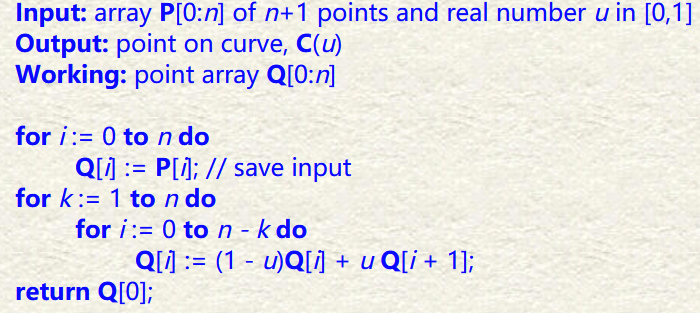
\includegraphics[width=9cm,height=4cm]{algorithm1.PNG}
	\caption{De Casteljau Bézier vertex evaluation algorithm}
\end{figure}
\\\indent 2.After setting the position of our control points to the surface,we start to evaluate the position and normal of the points sampled on the Bézier surface.Given any (u,v) ranging from [0,1]*[0,1], we can use the  algorithm demonstrated in Fig.2 to get the position of its corresponding point on the surface.
\begin{figure}[h]
	\centering
	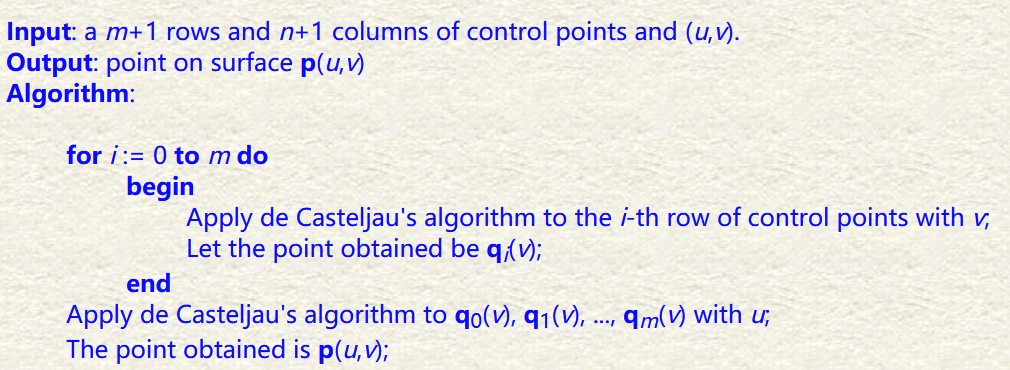
\includegraphics[width=9cm,height=4.5cm]{algorithm2.PNG}
	\caption{Position calculation of points on the Bézier surface}
\end{figure}
\\\indent To calculate the normal of the point,we have to calculate the tangent vector of the point along u and v direction first, and then calculate the cross product of these two vectors .As it is shown in Fig.3, in order to calculate the tagent, we have to note down the last two points which form the point we want, and minus their position. 
\begin{figure}[h]
	\centering
	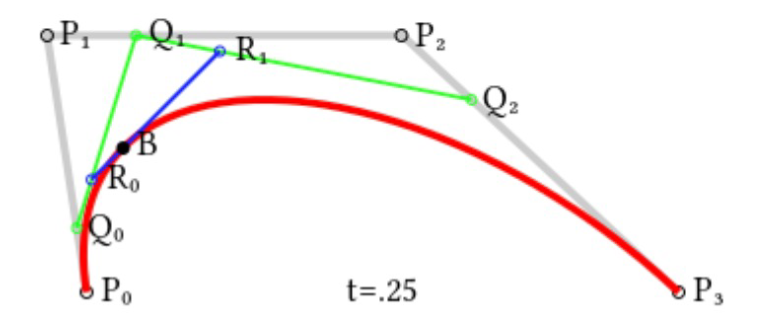
\includegraphics[width=9cm,height=4.5cm]{algorithm3.PNG}
	\caption{Tangent vector calculation}
\end{figure}
\\\indent 3.After finishing the procedure of how to calculate all the needed information for any (u,v) point, we evenly divide [0,1]*[0,1] into 64*64 grids,and each grid vertex is expressed as (u,v). Then we calculate all of those grid vertices and store their content into a vertex array, and set up the indices array which stores the sequence of every three points to construct the meshes.
\\\indent 4.In the stitching part, I stitch two Bézier surface patches together, maintaining 1st order continuity(i.e.not only the points are connected, but also their tangents are continuous at the joint.) To ensure this, we need to make sure that the control polygon are colinear at the last control point of the first surface and the first control point of the second surface. This can be achieved by setting the positions of the control points manually. 
\\\indent 5.To construct a B-spline surface, we first have to evaluate the position of a point on the B-spline curve given the control points,named as De Boor's algorithm. The algorithm is shown in Fig.4
\begin{figure}[h]
	\centering
	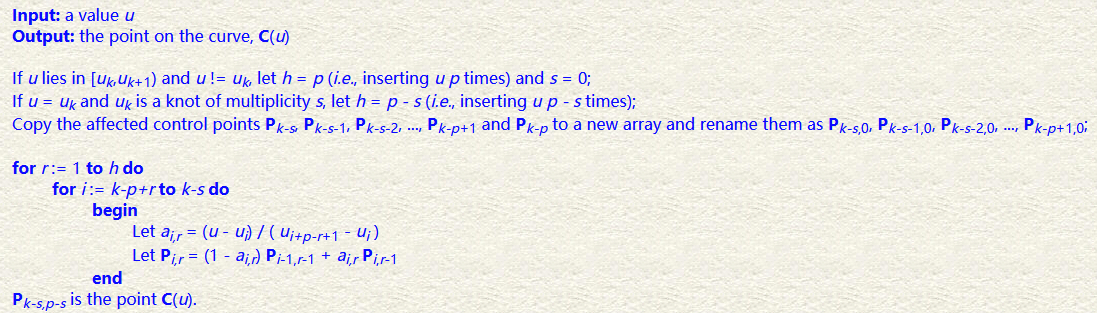
\includegraphics[width=9cm,height=4.5cm]{b_algorithm1.PNG}
	\caption{De Boor's algorthm}
\end{figure}
\\\indent Then it's relatively easy to find the position of a point on the B-spline surface based on De Boor's algorthm.The whole procedure is shown in Fig.5,and to tell the truth, the procedure is nearly as same as what we have done in constructing the Bézier surface.Therefore, the detailed information such as how to sample the points and construct the mesh is ommited in this step.
\begin{figure}[h]
	\centering
	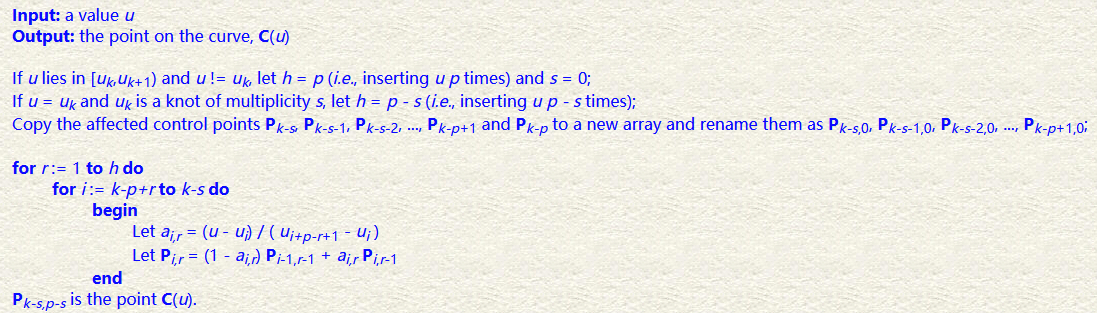
\includegraphics[width=9cm,height=4.5cm]{b_algorithm1.PNG}
	\caption{Position calculation of points on the B-Spline surface}
\end{figure}
\\\indent 6.To support the interactive editing (by selection) of control points,my method is that we should first store the position of current cursor,also the projection,view matrix, and then use the function glm::unproject() to backproject the screen position to 3d dimension.After that,compare this position to all control points' position so that we can find the nearest control point. Therefore, we can update the position of that control point to wherever we drag it in the next continuous frames. Also, after updation, we have to update the VAO,VBO of the surface in order to generate the updated surface.
\section{Results}
\qquad Below are the results of my programming work.Figure(a) to Figure(d) represent 'Single Bézier surface', 'Stitching Bézier surfaces', 'Bézier surface with moved controlpoints' and 'Single B-Spline surface' respectively.What's worth mentioning is that for Figure(d),my principle of selecting control points is to select 5*5 evenly distributed points on the planar surface, and move away the middle one of those points. The reason why I choose my control points in this way is that it can easily demonstrate the correctness of my B-spline surface realization,(also for the demonstration that my algorithm does not stuck into the poor condition that the surface converages into the zero point.)
\begin{figure}[htbp]
	\centering
	\subfigure[Single Bézier surface]{
		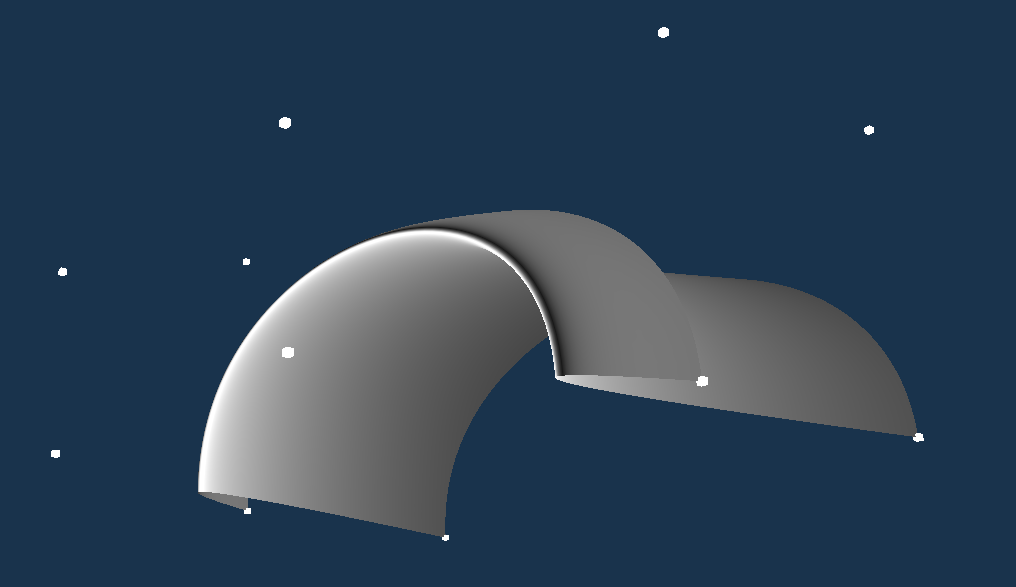
\includegraphics[width=3cm]{single.png}
		%\caption{Single Bézier surface}
	}
	\quad
	\subfigure[Stitching Bézier surfaces]{
		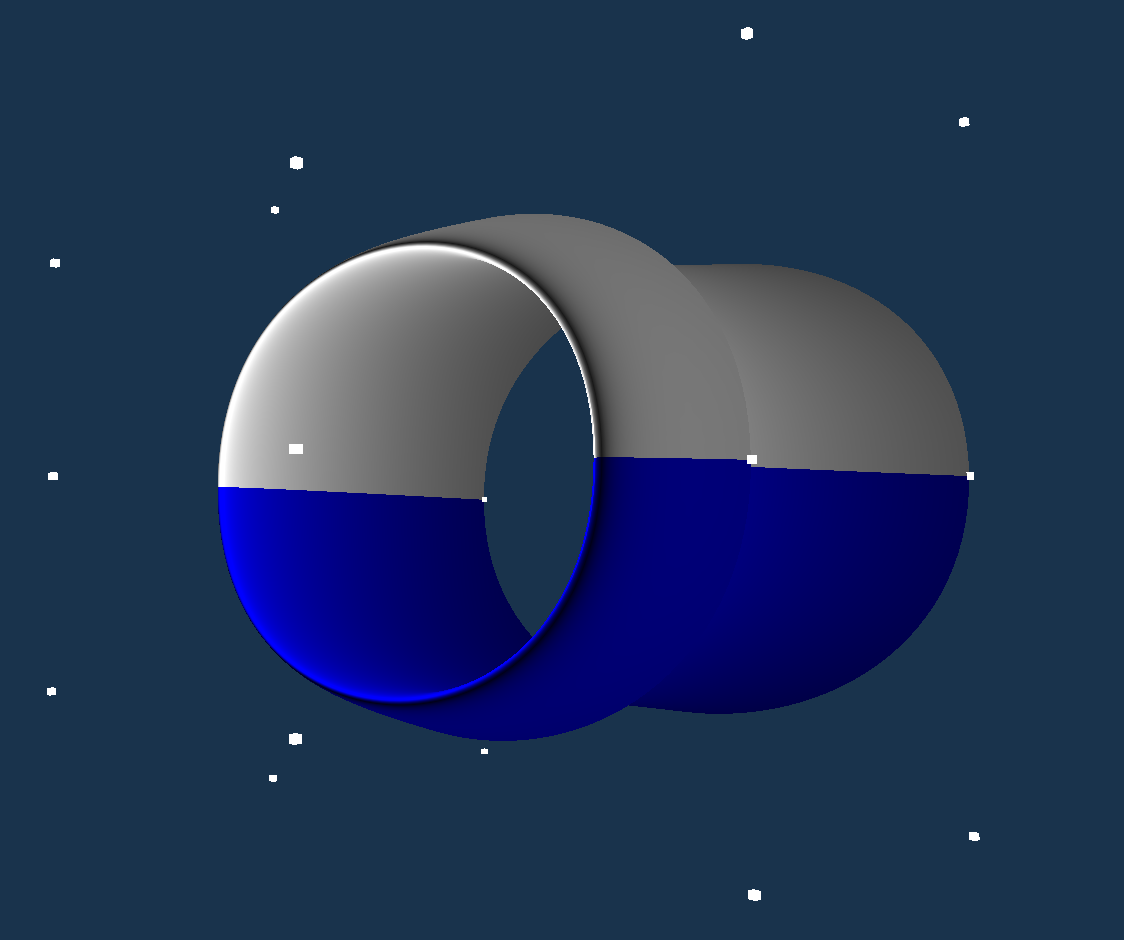
\includegraphics[width=3cm]{Stitching.png}
	}
	\quad
	\subfigure[Bézier surface with moved controlpoints]{
		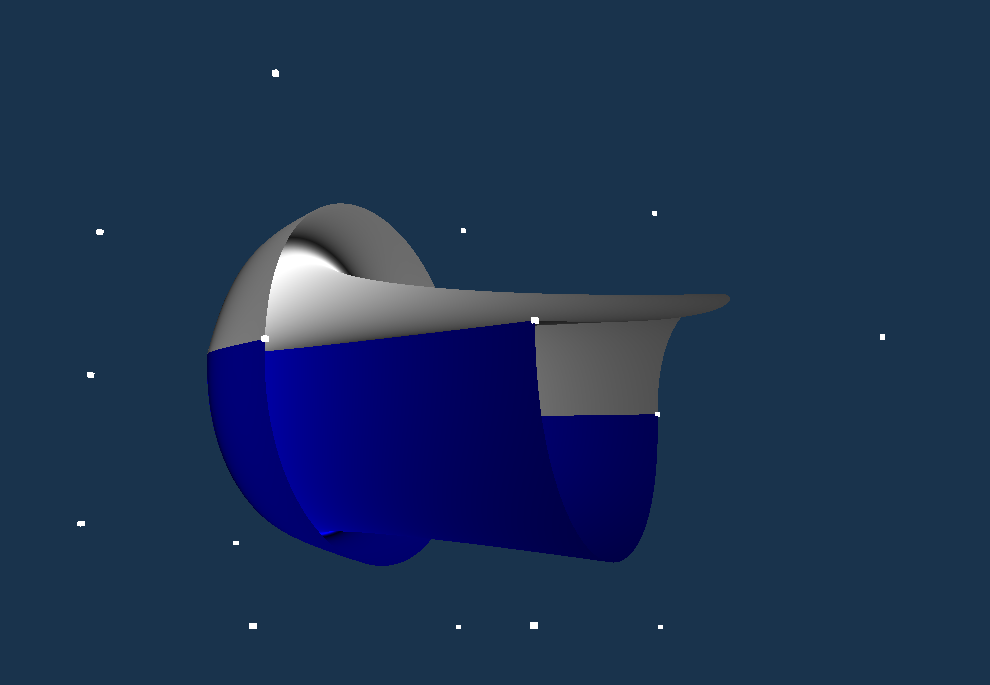
\includegraphics[width=3cm]{Move_control_point.png}
	}
	\quad
	\subfigure[Single B-Spline surface]{
		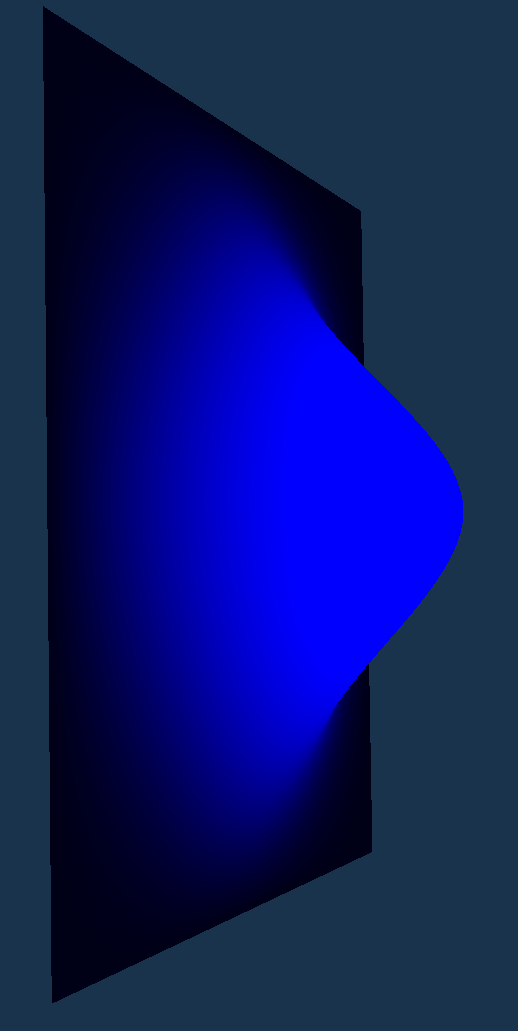
\includegraphics[width=3cm]{B-spline.PNG}
	}
\end{figure}
\end{document}
